\documentclass{report}

\usepackage{blindtext}
\usepackage[most]{tcolorbox}
\usepackage{graphicx}
\usepackage{float}
\usepackage{hyperref}
\usepackage[toc,page]{appendix}
\graphicspath{ {./Images/} }

\makeatletter
\NewDocumentCommand{\mynote}{+O{}+m}{%
  \begingroup
  \tcbset{%
    noteshift/.store in=\mynote@shift,
    noteshift=1.5cm
  }
  \begin{tcolorbox}[nobeforeafter,
    enhanced,
    sharp corners,
    toprule=1pt,
    bottomrule=1pt,
    leftrule=0pt,
    rightrule=0pt,
    colback=yellow!20,
    #1,
    left skip=\mynote@shift,
    right skip=\mynote@shift,
    overlay={\node[right] (mynotenode) at ([xshift=-\mynote@shift]frame.west) {\textbf{Note:}} ;},
    ]
    #2
  \end{tcolorbox}
  \endgroup
  }
\makeatother

\begin{document}

\title{Interim Report \\
\textit{3D Video Game: Hope and Control}}
\author{267533}

\maketitle

\section{Introduction}
While the written word can gain a form of dynamism through ambiguity, applying that to an interactive and visual medium becomes challenging to do concretely. Instead, gameplay elements, such as simulation and customisation, can be used to engender a narrative in the player, giving them the space to fill in the gaps in their own minds. When done well even non impactful decisions can be imbued with a sense of weight, this feeling that everything contributes. On the other end when done poorly, all decisions can become meaningless whether they are impactful or not. What matters is the player believing they're having an impact. 

This form of narrative interaction is seen commonly in the large-scale real-time strategy genre (e.g. Stellaris, Crusader Kings, etc.) where interlocking systems tell the stories of large factions. The objective of this project is to first create a beta version of a game in this genre, then perform a round of user testing. Insights gained from that process will then be used to complete a vertical slice. Given the constraints inherently imposed by solo development across such a limited time scale, it is unlikely a fully finalized version of the game will be completed.

To allow the player to make immediate, impactful decisions at the beginning of any given run, unlike most games in the genre, the player's power (i.e. their ability to affect the simulated environment) will be organized differently to the other factions. Instead of playing as a larger force the player will be a single powerful entity (i.e. a single ship, a single character, etc.) with a large amount of upfront ability to effect change. Alongside this, the player will be immediately presented with customization options for their faction typical to the genre (e.g. faction symbol, faction origin, etc.), leading them into a roleplaying headspace. 

To ensure that the player's actions result in dynamic outcomes, the faction simulation will also need to be suitably complex. As such, this project takes a code-agnostic, data driven approach. This involves keeping faction data separate from any given simulation element, as opposed to a typical object-oriented approach, which would intertwine them. This allows simulation modules to be designed and implemented in a flexible manner, as well as allowing extra simulation elements to be added easily as an extension goal.
\newline
\newline
This report consists of several sections, the first of which is "Professional Considerations", where user testing and acquiring consent for personal data collection is discussed in detail. Next is "Requirements Analysis", which outlines the objectives of the project in distinct steps alongside expanding on the explanation of the problem space and my solutions. This includes background research on games in the genre and proposed solutions to common game design issues. After that is "Art Design", which details some techniques used to render the large scale solar system, follwed by "Simulation Design". That section of the report discusses in detail all the parts that make up the simulation's structure, with some expansion on specific finer details.
Next is the "Project Plan", consisting of a breakdown of the work required to complete the project into distinct phases, illustrated using a Gantt chart. Then there is an "Interim Log" detailing the steps of the Project Plan completed as of the submission of this Interim Report. Finally, there are the bibliography and appendices.

\section{Professional Considerations}
\section{Requirements Analysis}

This poject aims to produce a player-story driven RTS (Real Time Stratergy). in the form of a vertical slice (a version of a game that lacks some features but still showcases what the final product will look like). Unlike a typical RTS, there will be a larger focus on the world reacting directly to the player as a singular powerful entity and less on long term historical stratergy. As such that world will need to be deeply simulated, comprising a large amount of the technical challenge of the project.
While the game will be in part targeted at long time RTS players, this change in power balance (alongside a shift into more roleplay focused elements of the genre) is designed to allow a wider audience to engage with a typically complex genre. 

This project uses Unity instead of a custom engine, the primary reason for this choice is my familiarity with it's workflow. I've previously created a full game using Unity (including shipping it to Steam) and I greatly enjoy its flexibility. Unity makes it easy to extend the editor through creating additional context menu items and entirely new editor tools. 
The C\# (which is Unity's primary coding language) ecosystem is also very broad, with a collosal number of resources to pull from. 

To assist with the development process, multiple rounds of in-person user testing should occur. The sample of players should be made up of both people familar with the RTS genre and those that are not, ideally spread evenly across that range. Two primary testing rounds should occur, one before an inital version of the game is produced and one afterwards, utilizing a beta version. This beta version can differ from the vertical slice dramatically in terms of completeness but should still be functional.
Any additional user testing (including online testing) is helpful but should be considered an extension objective given the time constraints.

\subsection{Background Research, Common Design Problems and Solutions}

\mynote{talk about how combat is handled as we refrence it in a later part of the document}

\subsubsection{Game 1: Stellaris}

Stellaris (2016) is a large scale space-based strategy game, taking place across a substantially sized galaxy. It involves managing an interstaller faction, taking them from their first ships to combating a galaxy wide threat. 

The game puts a heavy emphasis on roleplay right from the beginning of a run. Immediately upon selecting "New Game" you are presented with the screen pictured in Figure 1.

\begin{figure}[h]
    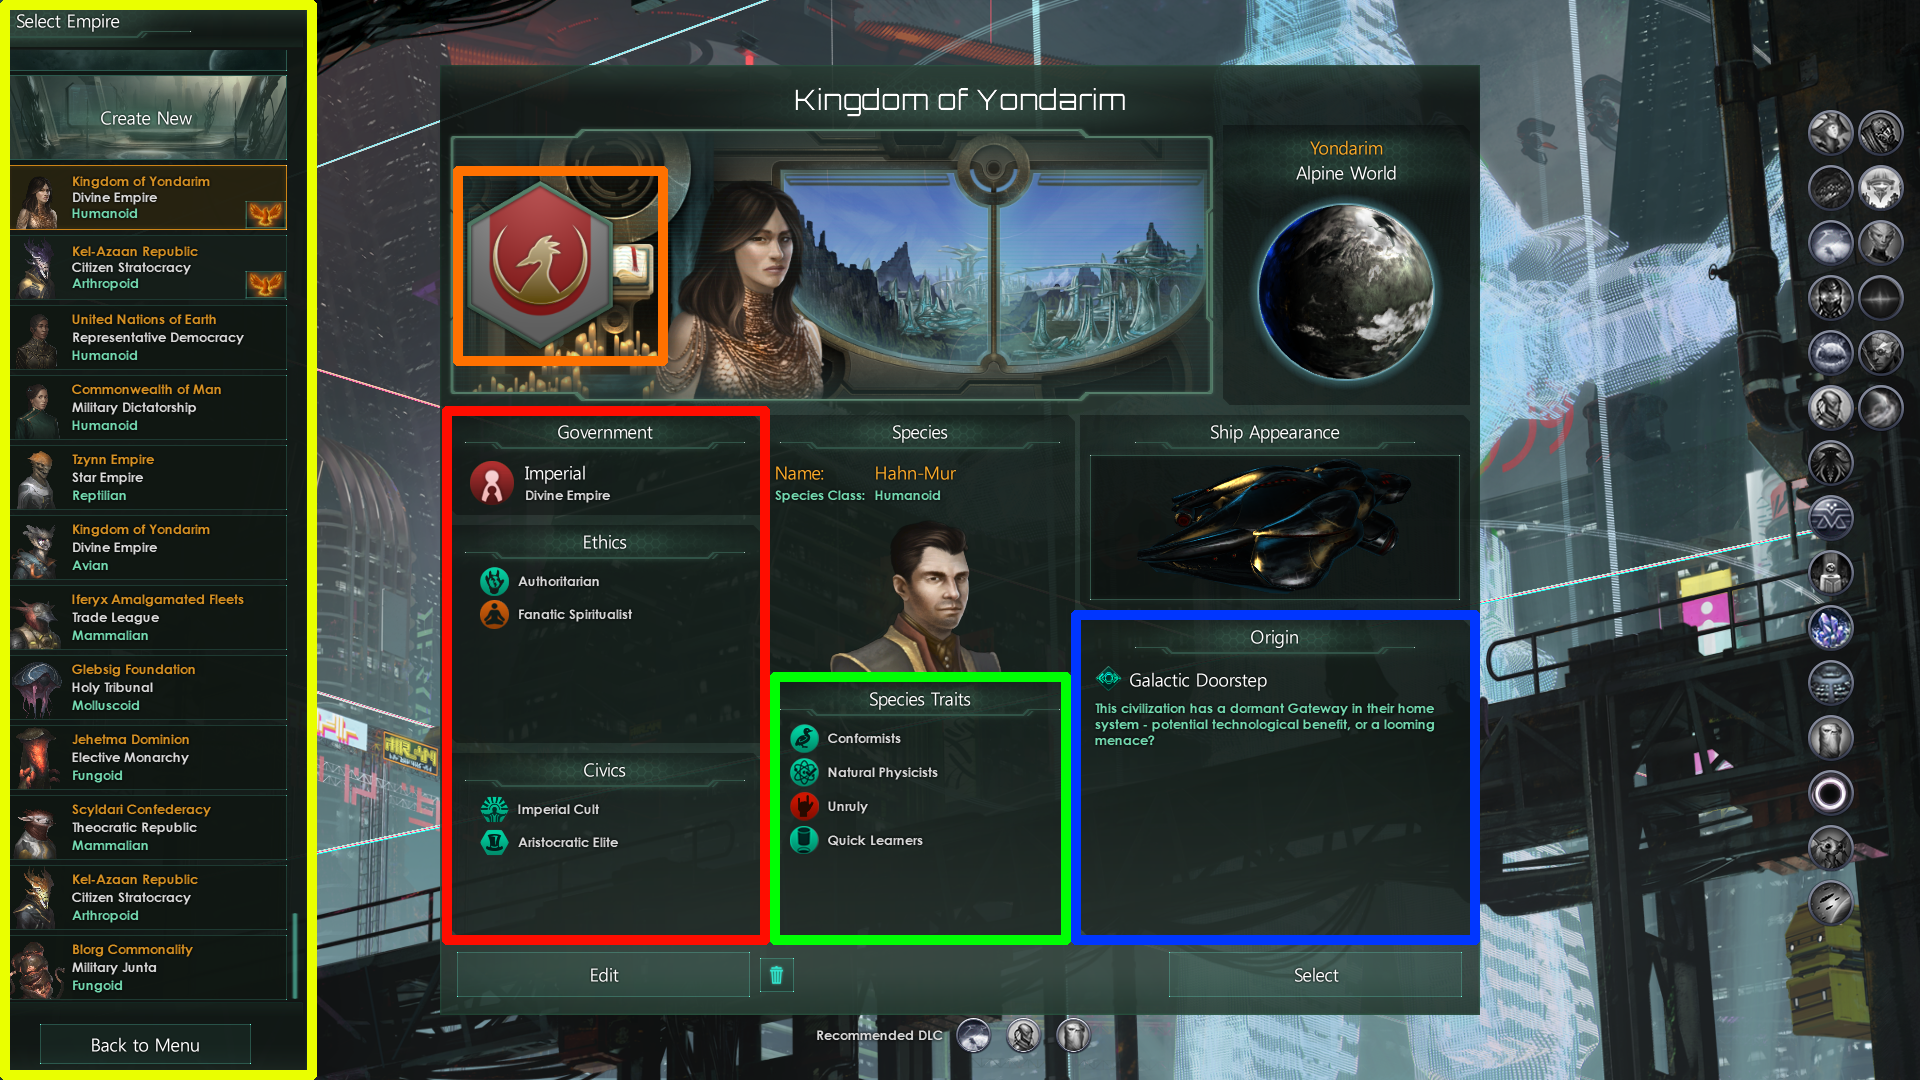
\includegraphics[width=\textwidth]{stellaris_faction_creation.png}
    \caption{Stellaris Faction Creation Screen}
\end{figure}

The left side of the screen showcases a list of premade factions (highlighted in yellow) that the player can pick from then customize, these can act as a  jumping off point for player ideas. There is additionally an option to create an entirely unique faction at the very top. 
Positioned diretly in the center of the screen is the information on the currently selected faction, including; their governmental practices (highlighted in red), their species traits (highlighted in green), their species origin (highlighted in blue) and their faction's flag (highlighted in orange). All these elements (alongside others) create a distinct feeling for this particular faction and, more importantly, they have gameplay ramifications. Within a minute of starting the game proper the faction shown in Figure 1. (an Imperial Divine Empire) was notified it had received a new heir, a special type of unit that acted (in this case) as a scientific advisor.

This focus on roleplay is reflected in the reviews for the game, many are simply retellings of their own faction's story. An example of this is pictured in Figure 2.

\begin{figure}[H]
    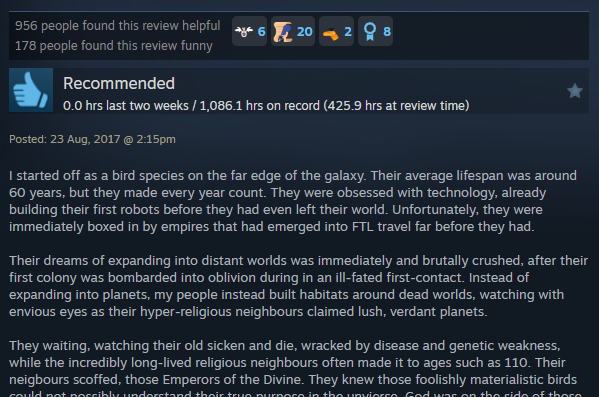
\includegraphics[width=\textwidth]{stellaris_positive_review.png}
    \caption{A retelling of a Stellaris game, (full review is 650+ words long)}
\end{figure}

Other systems also assist this storytelling, in particular the Galactic Crises. These are large, late game events that typically have ramifications for the whole galaxy and act as a definitive final boss for a playthrough. Interestingly, there are also specific cases where a player or AI can become the crisis, another avenue for potential roleplay. The player's relationship to other factions can be vitally important during these scenarios, meaning earlier (possible roleplay based) decisions can have a major impact.

Space combat is another important part of Stellaris but is more used as a tool to express roleplay decisions than a system that encourages roleplay itself. The functional act of combat instead enhances the grand stratergy side of the game, engagements are often won by decisions made before the battle starts. For example, the ships used by an endgame crisis, "Extradimensional Invaders", largely rely on shields as a defensive measure for their ships. This means that kinetic weapons are particular effective \cite{stellarisBattleDecision}, outfitting ships with these weapons is a decision made when they are created. When actually fighting, fleets of ships will "auto-battle" each other, with no input required by the player. While this project does focus more on a singular powerful entity, it will take a similar pre-planning approach to combat. This is in part due to the time constraints, as time spent making combat rewarding to execute takes time away from the simulation side (and main goal) of the project.
\newline
\newline
While Stellaris succeeds in many areas and is arguably (with it's balance of stratergy and roleplay) the closest real example of this project's goal, it has a few outstanding flaws. The game has a large amount of upfront complexity, the main Stellaris wiki's Beginner Guide \cite{stellarisBeginner} is roughly 17000 words long, split into 20+ sections and subsections. Figure 3. showcases the first screen players will see outside of the faction creation menu. It hosts a suite of information, shown to the player all at once. This includes (but is not limited too); eight types of basic resources, several more advanced resources (including fleet and starbase capacity), a list of all controlled entites (planets, fleets, construction and science ships and shipyards), the current date, many links to other UI windows (including Goverment Control, a larger galaxy map, Species Control, Technology and Research Management) and buttons for switching map mode (it should be made clear those buttons do nothing on this screen but are still present).

\begin{figure}[H]
    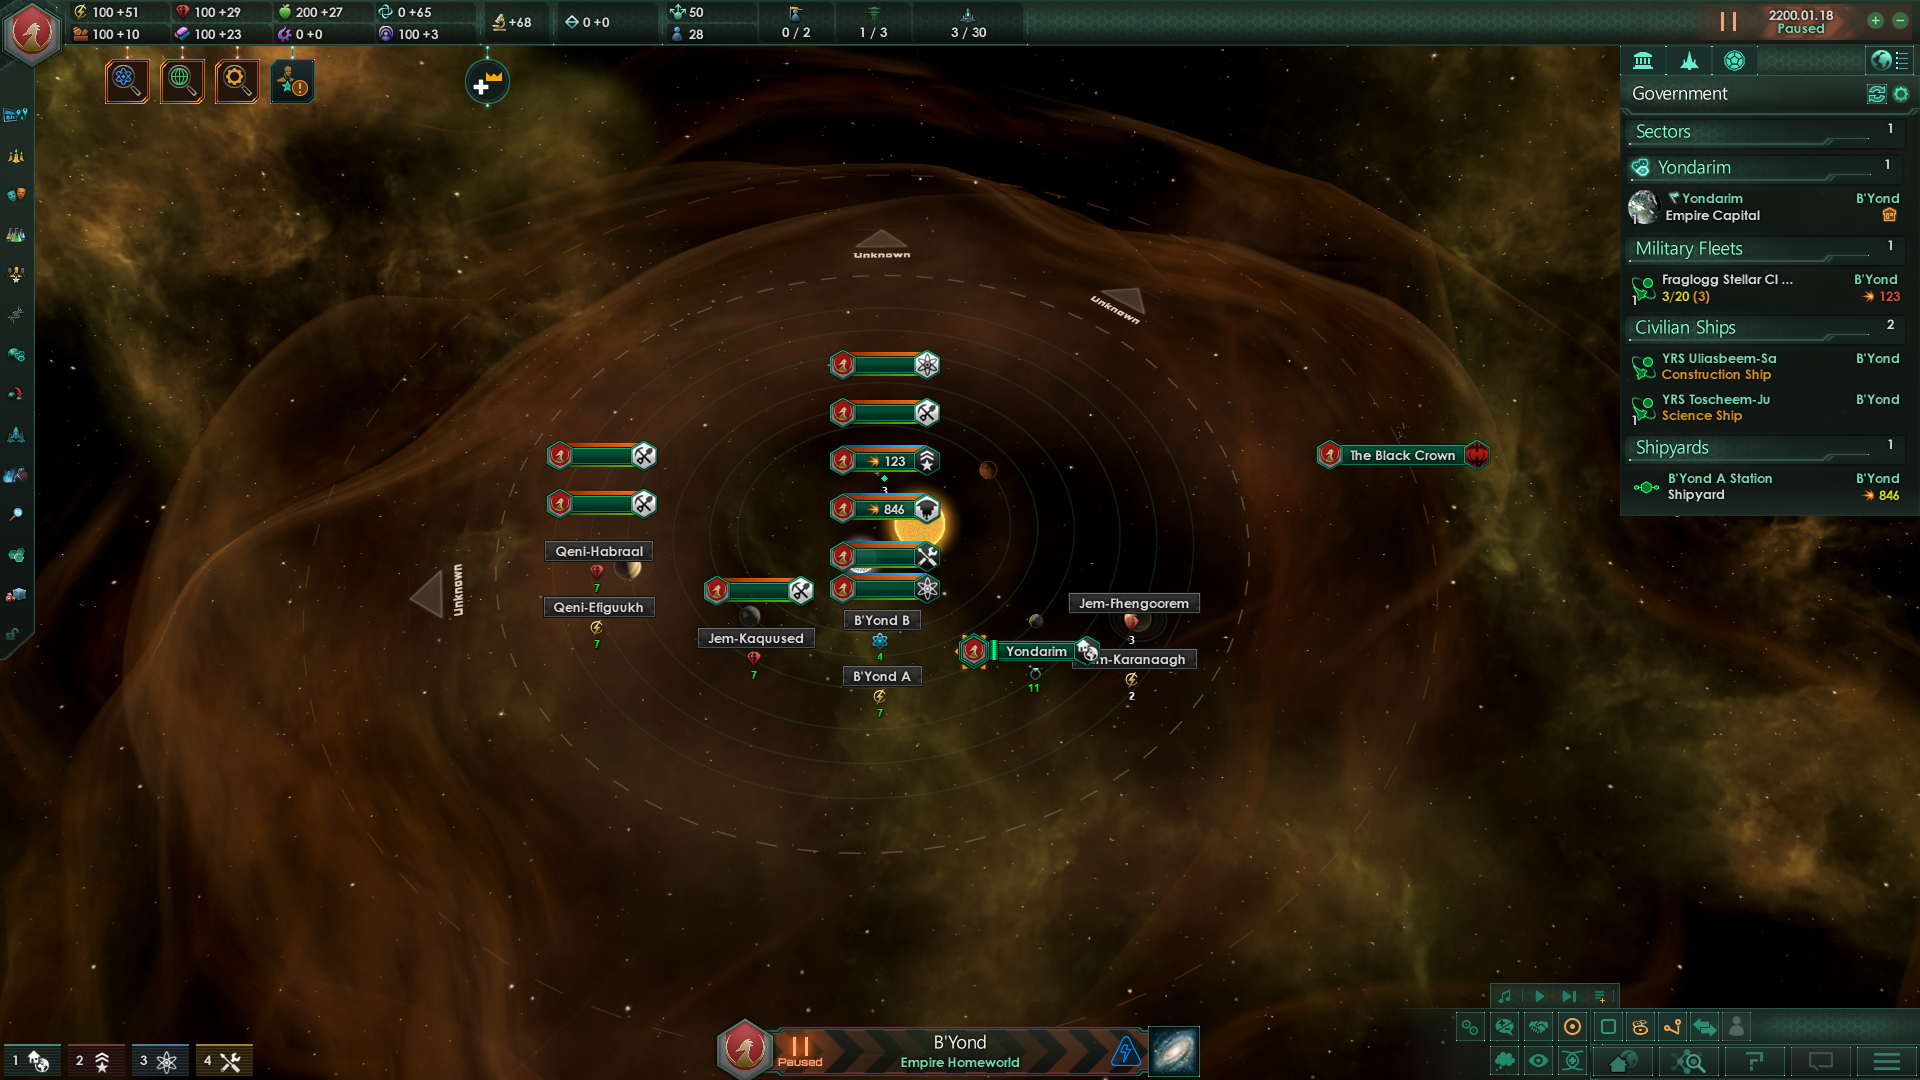
\includegraphics[width=\textwidth]{stellaris_main_screen.png}
    \caption{Stellaris Solar System View Screen}
\end{figure}

However, this complexity is an important, and arguably defining, part of the genre \cite{rtsUncertainty}. The principal issue here is how it is introduced to the player. Given this project's intention to, in part, target a wider audience, this issue is quite important. The intended solution is to introduce player elements gradually, in the context of the larger narrative brace of the game, this can be expressed as the player's controlled entity turning back on after many years inactive. To enhance replayability players could be allowed to start already in a fully active state rather than repeating the tutorial each time.

Stellaris also suffers from performance issues, particularly in the late game \cite{stellarisPerformanceReview1} \cite{stellarisPerformanceReview2}. Given the relative scales of this project and Stellaris this is a less relevant issue, performance goals are discussed further in the sub section "Performance and Stability".

\subsection{Performance and Stability}

Crashes and bugs should be kept to an ideal minimum. While the time constraints imposed don't allow the throughness typical of a standard project, ample time can still be allocated to unit testing and the like. The afformentioned rounds of user testing can also assist with this issue.

Alongside functioning as intended, the final version of the project should also run at a consistent and reasonable frame rate (60 frames per second) on low to medium range hardware. Given the relatively low intended visual complexity of the game, this objective is still important but easier to reach than others. Various different pieces of hardware are avaliable for testing, with varying hardware capabilities in each.

\subsection{Additional Gameplay Features}

If time allows, there are some additional gameplay features that would ideally be added;
\begin{itemize}
	\item Additonal simulation elements. For example, if the current version of the simulation models a planet's resources as a static value, a new simulation routine could decrease that value over time based on population and industrial activity.
	\item Online functionality. This would likely take the form of online leaderboards, showcasing statistics such as "Time Survived", "Enemies Killed", "Highest Bounty", etc.
	\item More advanced combat functionality, taking the form of additional actions ontop of the exisiting auto battle system. 
	\item Music. While many royalty free options exist, unique music would help set the mood properly for players.
	\item Releasing the game on Steam. Generally speaking this is a capstone objective and would signal the end of the code side of the project. 
\end{itemize}

\section{Art Design}

Visuals are an important part of game development but they are not the focus of this report. This section of the report will focus on the system used for large scale rendering (used for celestial bodies) as an example of some of the work done on that side of the game. 

The effect is made of two key parts, an "imposter sphere" shader and a system that converts real-space (As in the simulation position of the object being drawn) coordinates to a visual scale. 

\mynote{could talk about our system for displaying far away large things (shelled size based rendering)}

\section{Simulation Design}

\mynote{Use that draw.io diagram you made}
\mynote{Simulation is made up of Simulation Manager, Faction routines, Faction data, the Simulation Manager Execution Clamp and the faction drawer}

\section{Project Plan}
\section{Interim Log}

\begin{thebibliography}{9}
\bibitem{stellarisBeginner}
Stellaris Community, "Beginner's guide", "Stellaris WIki", 21 October 2024, \href{https://stellaris.paradoxwikis.com/Beginner\%27s_guide, Beginner's guide Link}{Beginner's Guide}
\bibitem{stellarisBattleDecision}
Stellaris Community, "Crisis/Endgame crisis factions/Extradimensional Invaders/Successfully repelling the Extradimensional Invaders", "Stellaris Wiki", 18 October 2024, \href{https://stellaris.paradoxwikis.com/Crisis#Successfully_repelling_the_Extradimensional_Invaders, Crisis Solution Link}{Extradimensional Invaders Stratergy}
\bibitem{rtsUncertainty}
Jónsson, B. Pages 6 to 7, "REPRESENTING UNCERTAINTY IN RTS GAMES"
\bibitem{stellarisPerformanceReview1}
Skullcrusher, "Stellaris Steam Review", "Steam", 11 September 2022, \href{https://steamcommunity.com/profiles/76561198026459371/recommended/281990, "Review Link"}{Link}
\bibitem{stellarisPerformanceReview2}
A Random Fish, "Stellaris Steam Review", "Steam", 18 October 2019, \href{https://steamcommunity.com/id/ARandomFish/recommended/281990. "Review Link"}{Link}
\end{thebibliography}

\begin{appendices}
\chapter{Project Proposal}
\noindent\makebox[\linewidth]{\rule{\paperwidth}{0.4pt}}
\begin{center}
\textbf{Space Based Simulation and Tactics Game}
\end{center}

\textit{Candidate Number: 267533}

\textit{Supervisor Name: Dr Paul Newbury}

\textbf{Aims}
\newline
Many games try to create a branching narrative. When done well this can imbue even non impactful decisions with a sense of weight, this feeling that everything contributes. On the other end, when done poorly, all decisions can become meaningless, whether they are impactful or not. What matters is the player thinking they’re having an impact.

In this project I intend to (with the constraints inherently imposed by solo indie development in mind) create a video game that creates an emergent narrative through gameplay rather than text, maximising the feeling of impact for the player. This form of narrative is seen commonly in the large-scale real-time strategy genre (e.g. Stellaris, Crusader Kings, etc.) where interlocking systems tell the stories of large factions. There will be some simplification to allow users that would normally be turned off by the upfront complexity of these games to also engage with the final product.

\textbf{Objectives}

\underline{\textit{Primary Objectives}}

\begin{enumerate}
	\item Research existing games in the genre, identifying their gameplay focus points \& style.
	\item Examine what games in the genre do well and what they do poorly.
	\item Conduct interviews with 5+ potential players, utilizing insights gained in Primary Objectives 1 and 2 to shape the questions asked
	\item Examine what games in the genre do well and what they do poorly.
	\item Use information from all Previous completed Objectives to design a game that tells player driven stories.
	\item Create a beta version of the completed game that can be tested and critically evaluated, both by me and potential players.
	\item Use insights gained from Primary Objective 5 to iterate and improve on the beta version.
	\item Ultimately finish a vertical slice that would lack some features but showcase accurately what the final product could look like.
\end{enumerate}

\underline{\textit{Extension Objectives}}

\begin{enumerate}
	\item Perform Primary Objectives 5 and 6 continuously to further improve the final product.
	\item Conduct critical evaluation using the vertical slice, in the same manner as Primary Objective 5.
	\item Utilize the insights gained in Extension Objective 2 to further improve upon the vertical slice, expanding it into a fully completed game.
	\item Implement additional simulated features into the game, refining the model.
	\item Implement online leaderboard functionality for various statistics.
	\item Release the fully completed game on platforms such as Steam and Itch.io.
\end{enumerate}

\textbf{Relevance}

This project reflects my intended career path, as someone that has already been working with Unity and C\# for the last five years. During my gap year (2021 - 2022) I went through the full development process, releasing a 2D game on Steam in early July. Since then, I’ve been working on both my development and 3D skills and hope to release another game I’ve been working on a couple months post university.

By doing this project I hope to further both my coding and artistic skills, combing them to create a hopefully great video game. This project tests both of those disciplines alongside my ability to gather effective feedback and implement proper HCI principles.

\textbf{Resources Required}

I will require use of study rooms/seminars to conduct in person user testing. Testing will also be conducted online but that should require minimal resources. No funding will be required as I expect to purchase games used for market research myself. I also expect to pay for the Steam direct fee if Extension Objective 6 is completed.

Some use of lab computers is required (primarily on Mondays) though I intend to use my home PC on a day-to-day basis. This is due to several factors; my extensive backlog of previous projects I can pull reusable systems/assets from, the comfortability of the workspace and the ease of access, alongside various others.

\textbf{Time Management}

\begin{table}[htbp]
\begin{tabular}{|c|c|c|c|c|c|c|c|}
\hline
 & Monday & Tuesday & Wednesday & Thrusday & Friday & Saturday & Sunday \\
\hline
9:00 &&&&&&& \\
\hline
10:00 & Lecture & & Lecture &&&& \\
\hline
11:00 & \textbf{Project} &&&&&  \textbf{Project} &  \textbf{Project} \\
\hline
12:00 & \textbf{Project} & & \textbf{Project} & \textit{Seminar} & \textbf{Project} & \textbf{Project} & \textbf{Project} \\
\hline
13:00 & Lab & Lecture &  \textbf{Project} & &  \textbf{Project} &  \textbf{Project} &  \textbf{Project} \\
\hline
14:00 &&&&&&& \\
\hline
15:00 & Lecture & & & Lab & Lecture && \\
\hline
16:00 & Lecture & & & Lab & Lecture && \\
\hline
\end{tabular}
\label{tab:schedule}
\end{table}

Project time per week is equal to 12 hours. This acts as a minimum goal and (due to my general passion for the subject matter) I will likely do more depending on the week. Any blank slots will be used for other modules, whether coursework or study. The minimum time spent each week will increase depending on unseen factors such as unintended scope creep or hidden complexity.

I intend to have the initial early beta version of the finished shortly after the interim report (Week 8 to 9 of Term 1), utilizing feedback gained over the Christmas break. I then expect to finish the final vertical slice a couple weeks before the final report is due. Any additional time gained, by being ahead of schedule, will be used to complete extension objectives, primarily Extension Objectives 1 and 2.

\noindent\makebox[\linewidth]{\rule{\paperwidth}{0.4pt}}

\begin{center}
\textbf{This proposal has been adapted from Word to \LaTeX{}, so exact formatting differs from the original proposal document. Structure and content remains the same.}
\end{center}
\end{appendices}

\end{document}